\documentclass[11pt,a4paper]{article}
\usepackage[utf8]{inputenc}
\IfFileExists{glyphtounicode.tex}{\input{glyphtounicode.tex}}{}
\pdfgentounicode=1
\usepackage[margin=22mm]{geometry}
\usepackage{graphicx}
\usepackage[hidelinks]{hyperref}
\usepackage{url}
\setlength{\emergencystretch}{4em}
\setlength{\parindent}{0pt}
\setlength{\parskip}{6pt}
\begin{document}
\title{VL405: Scan-Based Low-Switching LBIST for cMIPS32}\author{VL405 Project Submission}\date{}\maketitle\tableofcontents\clearpage


\textbf{Timing revision:} PASS: constrained OOC setup/hold/pulse and unconstrained-path checks. The latest analysis at 9.756097561 MHz is documented in \href{FPGA_Analysis/Timing_Closure/README.md}{Timing\_Closure}. Earlier 50 MHz tables below remain labeled historical evidence.



\textbf{Final submission report --- repository S4K50M/LBIST.} Historical implementation baseline: commit \texttt{2c9b90c} (Phase 6A). Target: Basys 3 Artix-7 \texttt{xc7a35tcpg236-1}; tool: AMD Vivado/XSim 2025.1.1. All numerical experiment results below are derived from retained native logs/CSVs. FPGA figures use the final native reports, with analysis stage explicitly identified.



\section{Abstract}


This project implements and verifies a programmable pseudorandom scan-test system around one 64-bit IF/RF pipeline register in cMIPS32. A 16-bit LFSR, combinational phase shifter and dynamic PLPF supply Direct, constant n=3, Basic, Swap and Moving approaches. Processor isolation protects architectural state while a controller performs 64 SHIFT, one CAPTURE and 64 UNLOAD edges per pattern. A completion-safe 16-bit MISR compresses actual serial responses. With 256 patterns, every initial approach detects 12 of the same 16 capture-input stuck-at faults, with no observed final-signature alias. Measured SHIFT WTM spans 7.0665\%--50.1154\%. These are simulation switching metrics; the FPGA power study is a separate tool estimate. The results establish this limited capture-cone experiment, not whole-processor fault coverage or measured physical power savings.



\section{Introduction and problem statement}


Scan shifting can cause sustained internal transitions. Filtering pseudorandom stimulus offers a controllable activity tradeoff, but it must preserve scan ordering, functional behavior, capture timing and response integrity. The project asks whether the existing filter/control approaches can operate on real cMIPS pipeline storage with reproducible results and safe error handling. The submission freezes the verified Phase 6A architecture. It adds production integration wrappers, final verification, reporting and FPGA analysis; no additional scan chain or fault site is introduced.



\section{Reference paper and proposed methodology}


Kato, Wang, Sato, Kajihara and Wen [1] motivate programmable scan-in activity using modified pseudorandom patterns. This project evaluates that principle on cMIPS. It reuses the established Basic/Swap/Moving schedules and independently checks every applied scan bit. The RTL uses counters and combinational decoders; it does not claim the paper's exact gate structure, silicon area, TEG measurements or general fault-coverage results. This report's measured values come from the repository's own experiment evidence.



\section{cMIPS32 architecture}


cMIPS is a five-stage VHDL processor: instruction fetch, register fetch, execute, memory and writeback [2]. Pipeline boundaries are \texttt{reg\_IF\_RF}, \texttt{reg\_RF\_EX}, \texttt{reg\_EX\_MM} and \texttt{reg\_MM\_WB} in \texttt{cMIPS/vhdl/pipestages.vhd}. The original functional core, exception/control logic and register storage are preserved. \texttt{docs/scan\_register\_inventory.csv} records widths, resets, types and scan decisions. Boolean/enumerated state needs deliberate encoding; it is not silently flattened into the implemented chain. The remaining 656 pipeline candidate bits are unscanned.



\section{LBIST system architecture}


\begin{figure}[htbp]\centering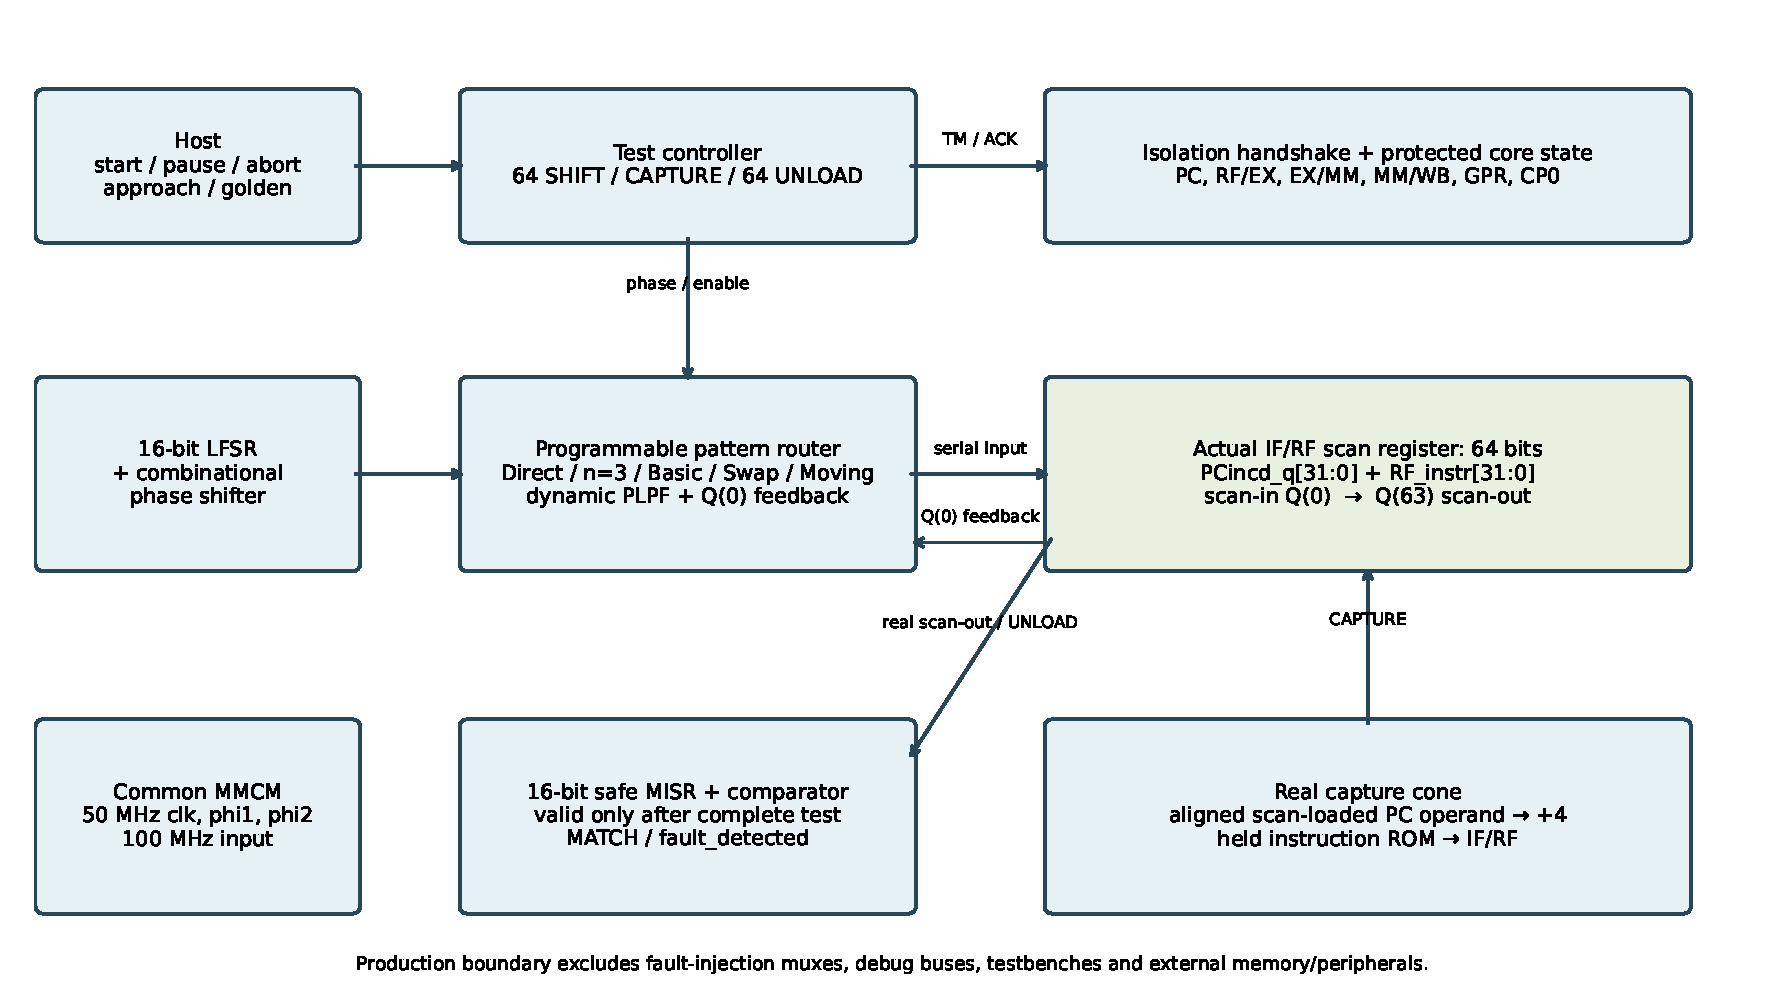
\includegraphics[width=\textwidth,height=.67\textheight,keepaspectratio]{figures/architecture.pdf}\caption{Production architecture}\end{figure}


\texttt{final\_processor\_system.vhd} selects original core (A), scan/isolation core (B), or the complete programmable LBIST core (C). C instantiates the verified controller, router, \texttt{core\_scan\_test} and safe MISR. Real scan Q(0) feeds the filter and Q(63) supplies the analyzer. Approach and golden signature are external configuration inputs held stable throughout a test. Test mode remains a real runtime control. Fault injection and wide debug probes are absent from production C; observation outputs on the core are open.



\section{LFSR and phase shifter}


The polynomial is x\textasciicircum{}16+x\textasciicircum{}15+x\textasciicircum{}13+x\textasciicircum{}4+1. State bit i denotes sequence position j+i; output is state(0), and feedback is state(15) XOR state(13) XOR state(4) XOR state(0). Reset seeds AAAA; zero/unknown seed protection is retained. The period bench checks all 65,535 unique nonzero states, sequence recurrence, bit balance, pause, resume and reset. The phase shifter exposes state(0), state(1), state(2) as current/next/next-next without extra cycles. The integrated experiment uses one scan chain; historical multi-chain standalone tests do not imply multiple processor scan chains.



\section{PLPF design and WTM control}


The dynamic PLPF is combinational. Mode 11 passes the current LFSR bit (n=1). Mode 01 combines two consecutive bits and real scan-input-stage feedback (n=2). Mode 00 similarly uses three bits (n=3). For feedback zero, the selected bits are ANDed; for feedback one they are ORed. Invalid mode holds feedback and raises invalid status. There is no extra shift for mode changes.



Measured WTM = 100 $\times$ sum over 256 patterns, 64 SHIFT edges and physical stages k of (k+1) $\times$ [Q\_k changes], divided by 256 $\times$ 64 $\times$ 2080. Input-stage weight is 1 and output-stage weight is 64. CAPTURE and UNLOAD transitions are excluded from this metric. Serial toggle rate and unweighted scan-FF switching are separate CSV columns. Theoretical WTM is an optimization estimate, not an assertion that a finite deterministic sequence reaches an arbitrary requested target.



\section{Basic, Swap and Moving controllers}


Basic beta=20 uses physical regions alpha/beta/gamma=22/20/22. Physical order is scan-in $\rightarrow$ alpha $\rightarrow$ beta $\rightarrow$ gamma $\rightarrow$ scan-out; chronological injection reverses it. Swap beta=16 alternates gamma=32 and 16 on successive captured patterns. Moving beta=20 uses gamma=14+p mod 17 and alpha=64-20-gamma. The minimum 14-cell filtered ends restrict the reachable unfiltered region. The offline optimizer chooses legal integer lengths; it is not on-chip optimization hardware.



Swap and Moving have separate SHIFT and UNLOAD scheduling instances. Both process schedule p; only the next SHIFT uses p+1. This avoids double-advancing the schedule during disposable unload shifts. LFSR state advances on every accepted SHIFT or UNLOAD, and holds during CAPTURE/pause. C's shared runtime router uses beta=20 and Swap beta=16 for all five modes; changing runtime mode does not change synthesized area.



\section{Scan-chain insertion}


Only IF/RF is replaced by verified \texttt{reg\_IF\_RF\_scan}: 32 PC-increment bits plus 32 instruction bits. The combined word is PCincd\_q \& RF\_instr, with serial insertion at bit0, output at bit63 and MSB-first unload. Scan disabled reproduces original load/reset behavior. The unit bench checks all 64 positions, feedback, reset, load/hold and scan priority. Native original-versus-scan processor regression compares internal pipeline values and functional buses under lwsw and memory stalls.



\section{Processor test-mode isolation}


Entry waits for idle external fabric and synchronized phase acknowledgements. The isolation boundary holds PC, downstream pipeline registers, general registers, exception/CP0 storage and side effects. Memory and register write attempts are monitored; committed writes remain suppressed. Only a legal CAPTURE updates IF/RF. Tests perturb interrupts, waits, errors, readiness, pause and attempted early exit. Exit is reset-only; arbitrary resume from destructively shifted IF/RF state is unsupported. Autonomous external peripherals are outside the protected core boundary.



\section{MISR response compression}


The analyzer polynomial is x\textasciicircum{}16+x\textasciicircum{}12+x\textasciicircum{}5+1 (mask 1021), seed zero. Each UNLOAD edge uses actual pre-shift scan\_out. The last response bit updates the signature before comparison settles. Phase 6A validity requires DONE phase 101, successful controller completion, 256 captures, 16,384 response bits, 256 complete unload words, matching controller pattern count and no sticky stream/controller error. MATCH and fault\_detected stay low until signature\_valid. A completed faulty stream is valid and may mismatch; abort/incomplete streams cannot claim MATCH. Eight safety scenarios cover normal/faulty completion, abort in each active phase, missing response, illegal restart and reset. Historical unsafe Phase 5B files remain unchanged for provenance and are not used in production C.



\begin{figure}[htbp]\centering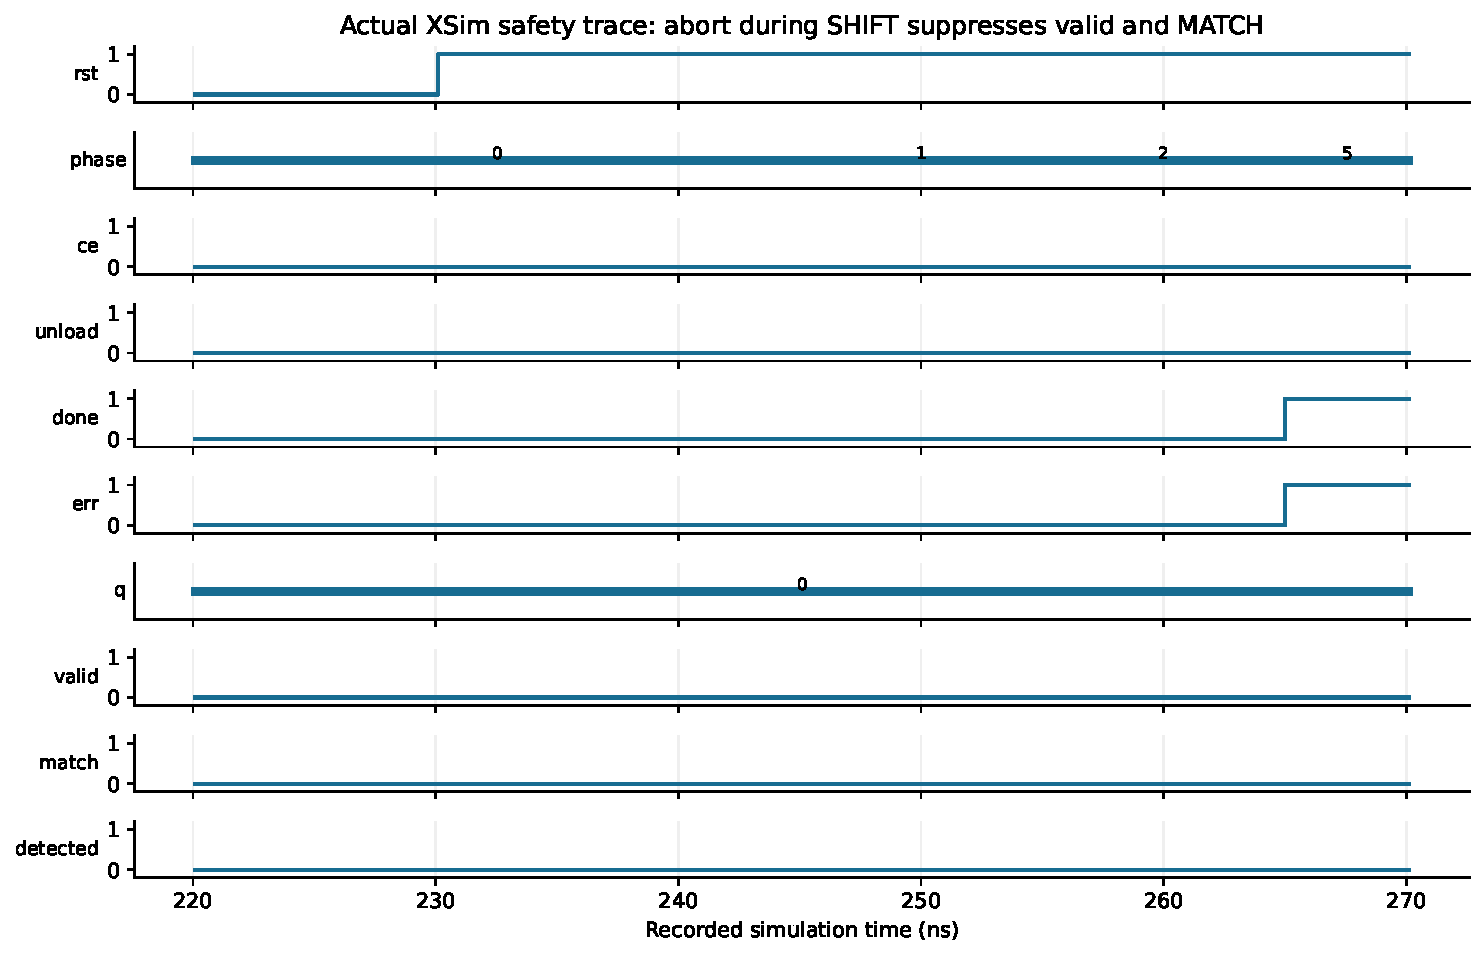
\includegraphics[width=\textwidth,height=.67\textheight,keepaspectratio]{figures/misr_abort_trace.pdf}\caption{Abort does not produce a valid signature}\end{figure}


\section{Fault-injection methodology}


The primary universe contains eight sites $\times$ SA0/SA1: increment\_operand bits 2,3,16,31 before the original +4 adder, and instruction\_input bits 0,1,16,31 before IF/RF capture. Fault muxes act only during legal CAPTURE. Injection is on real capture inputs, not scan-output corruption. Upper response is the aligned scan-loaded operand plus4 through the original processor adder; lower response is actual held-ROM instruction 1460FFFA at PC 2 C. Other processor logic remains held. This small cone is not the full datapath, ALU or instruction-set universe. Detected IDs are 1--8,10,11,14,16; IDs 9,12,13,15 have the already-held instruction polarity and are not excited. \texttt{tables/fault\_inventory.csv} supplies exact sites and activation paths.



\section{Verification and experimental setup}


All accepted simulations remain below 100 ms simulated time. The original 50 MHz, 256-pattern processor experiments finish at 661.6002 us. The fresh clock-revision experiments finish at 3.390701025 ms at 9.756097561 MHz; their nine-case summary is included in the timing revision below. Original Phase 1--6A artifacts are retained. Finalization rechecks the archived 204 experiments against independent stimulus/response/MISR/activity models, rather than rewriting historical campaigns. Fresh native tests exercise generator/filter/controllers, scan, isolation, safe analyzer/router, functional equivalence, and production C against the verified reference. The production fixture checks functional ports, real scan interface and analyzer outputs at all CPU phases, while recording its own switching activity.



\begin{center}\resizebox{\textwidth}{!}{\begin{tabular}{lll}\hline

\textbf{Category} & \textbf{Passed} & \textbf{Total} \\\hline
Fresh essential XSim & 13 & 13 \\
Fresh production equivalence/activity & 5 & 5 \\
Fresh original/production-scan functional activity & 1 & 1 \\
Fresh representative original-universe fault & 1 & 1 \\
Fresh native WDB/WCFG pairs reopened & 6 & 6 \\
Archived processor experiments independently rechecked & 204 & 204 \\
Archived waveform figures rechecked against VCD & 45 & 45 \\
Earlier files unchanged by SHA-256 & 2486 & 2486 \\
\hline\end{tabular}}\end{center}


The expected original \texttt{RF\_STOP\_SIMULATION} assertion at breakpoint PC00000038 terminates lwsw. It counts as success only with matching differential state, the exact breakpoint and ten printed values FFFFFFF6\ldots{}FFFFFFFF. Other failures are rejected. The old incomplete sixteen-replica Moving native attempt is excluded; its smaller retries provide complete accepted records. Fresh script errors, if any, remain in execution logs and are not relabeled as simulation passes. See \texttt{Verification/} and \texttt{final\_verification\_summary.md}.



\section{WTM results}


\begin{center}\resizebox{\textwidth}{!}{\begin{tabular}{llllllll}\hline

\textbf{Approach} & \textbf{Beta} & \textbf{WTM} & \textbf{Coverage} & \textbf{Golden} & \textbf{Aliases} & \textbf{Patterns} & \textbf{Cycles} \\\hline
Direct & fixed & 50.1154\% & 12/16 & 9A6A & 0 & 256 & 33024 \\
Constant n=3 & fixed & 7.0665\% & 12/16 & 5DCB & 0 & 256 & 33024 \\
Basic & 20 & 19.9764\% & 12/16 & AFBC & 0 & 256 & 33024 \\
Swap & 16 & 17.7531\% & 12/16 & 9C7F & 0 & 256 & 33024 \\
Moving & 20 & 19.8701\% & 12/16 & F21E & 0 & 256 & 33024 \\
\hline\end{tabular}}\end{center}


\begin{figure}[htbp]\centering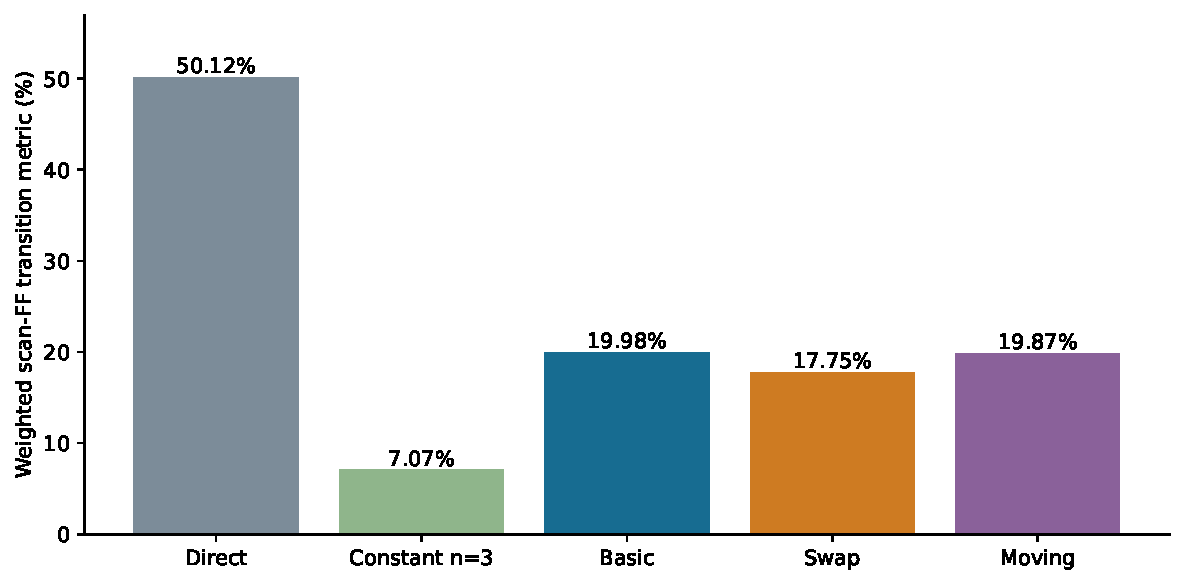
\includegraphics[width=\textwidth,height=.67\textheight,keepaspectratio]{figures/wtm_comparison.pdf}\caption{Measured WTM}\end{figure}


\begin{figure}[htbp]\centering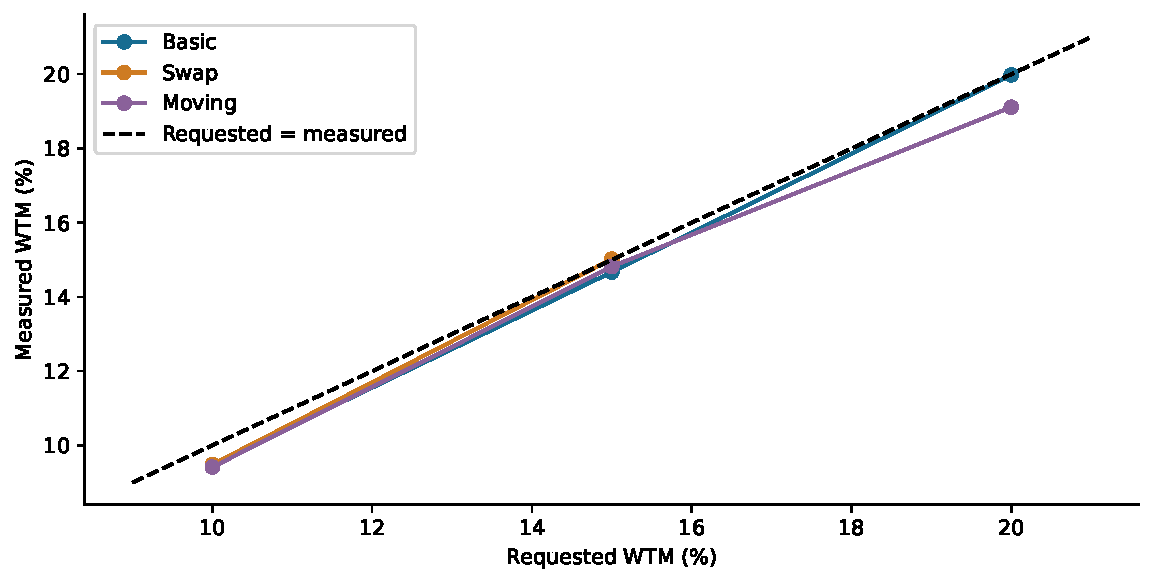
\includegraphics[width=\textwidth,height=.67\textheight,keepaspectratio]{figures/target_vs_measured.pdf}\caption{Requested and measured WTM}\end{figure}


\begin{center}\resizebox{\textwidth}{!}{\begin{tabular}{llllll}\hline

\textbf{Approach} & \textbf{Target} & \textbf{Beta} & \textbf{Estimate} & \textbf{Measured} & \textbf{Within 0.5 pp} \\\hline
Basic & 10 & 4 & 9.8214 & 9.4801 & False \\
Basic & 15 & 12 & 15.1786 & 14.6669 & True \\
Basic & 20 & 20 & 20.5357 & 19.9764 & True \\
Swap & 10 & 4 & 9.8214 & 9.4866 & False \\
Swap & 15 & 12 & 15.1786 & 15.0168 & True \\
Swap & 20 & 18 & 19.1964 & NOT\_RUN (infeasible) & False \\
Moving & 10 & 4 & 9.8214 & 9.4148 & False \\
Moving & 15 & 12 & 15.1786 & 14.8169 & True \\
Moving & 20 & 19 & 19.8661 & 19.1090 & False \\
\hline\end{tabular}}\end{center}


Target 10\% optimizer configurations achieve 9.4148--9.4866\%: close to one another but outside the declared $\pm$0.5 percentage-point target tolerance. At 15\%, Basic/Swap/Moving achieve 14.6669/15.0168/14.8169\%, respectively. Swap 20\% is infeasible with the legal L64 bounds; nearest beta 18 estimates 19.1964\%. Moving beta 19 is the optimizer-selected 20\% candidate and measures 19.1090\%; the separately tested beta 20 calibration measures 19.8701\%. Neither is relabeled. All exact feasibility and pairwise match decisions are retained in \texttt{tables/feasibility.csv} and \texttt{tables/matched\_comparisons.csv}.



\section{Fault-coverage results}


\begin{figure}[htbp]\centering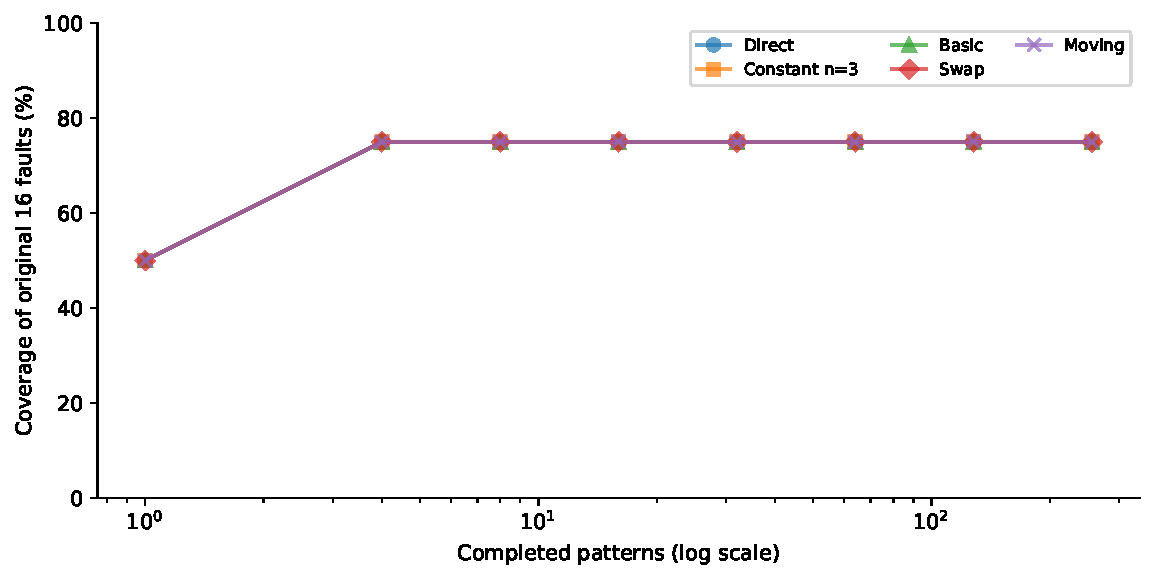
\includegraphics[width=\textwidth,height=.67\textheight,keepaspectratio]{figures/fault_coverage.pdf}\caption{Original fault coverage}\end{figure}


All five initial approaches reach 75\% of the 16 eligible capture-input faults after four complete patterns. All retain 12/16 direct and final-MISR detections at 256 patterns. No final alias is observed in these deterministic experiments. Four unexcited faults produce equal direct responses and equal signatures; they are not aliases. A 16-bit signature still has a finite alias risk for other responses and workloads; zero observed aliases is not proof of zero alias probability. The complete80 primary faulty signatures, first direct/prefix-MISR detection indices and outcomes are retained in the campaign/aliasing CSVs. Additional measured target profiles are secondary evidence and preserve the same denominator.



\section{Test-time analysis}


\begin{center}\resizebox{\textwidth}{!}{\begin{tabular}{lllllllll}\hline

\textbf{Approach} & \textbf{Detected} & \textbf{Undetected} & \textbf{First direct min} & \textbf{First direct max} & \textbf{Mean (detected)} & \textbf{Patterns to 75\%} & \textbf{Cycles to 75\%} & \textbf{Full cycles} \\\hline
Direct & 12 & 4 & 1 & 4 & 1.7500 & 4 & 516 & 33024 \\
Constant n=3 & 12 & 4 & 1 & 4 & 1.7500 & 4 & 516 & 33024 \\
Basic & 12 & 4 & 1 & 4 & 1.5833 & 4 & 516 & 33024 \\
Swap & 12 & 4 & 1 & 4 & 1.5833 & 4 & 516 & 33024 \\
Moving & 12 & 4 & 1 & 4 & 1.6667 & 4 & 516 & 33024 \\
\hline\end{tabular}}\end{center}


Each test executes 256 $\times$ (64+1+64)=33,024 payload cycles:16,384 SHIFT,256 CAPTURE,16,384 UNLOAD. The native experiment has 33,080 rising edges, including 3 paused and 53 other setup/handshake/exit/reset/restart overhead edges. Completion is 200 ps after its final falling edge. Payload time at 50 MHz is 660.48 us; the full bench duration is 661.6002 us. The power window separately spans 610 ns--661150.001 ns, covering the complete payload plus the three pauses and excluding reset/restart. Threshold 516 cycles is an observed coverage prefix; the actual runs still execute all 256 patterns. The architecture uses non-overlapped unloading, so it does not claim an overlapped test-time improvement.



\section{FPGA Implementation, Area Overhead and Power Estimation}


\textbf{Historical 50 MHz baseline:} The following original tables are preserved. The timing revision later in this section contains the current matched implementations.



\subsection{Comparable hardware and implementation boundary}


Vivado's installed part database confirms \texttt{xc7a35tcpg236-1}. Native synthesis obtains the Artix-7 license; no paid-only device or IP is selected. Configurations share source versions, flattened/rebuilt out-of-context synthesis, default optimization/place/phys-opt/route settings and common clock/reset infrastructure. A instantiates original \texttt{core}; B instantiates \texttt{core\_scan\_test} with an external tester interface; C adds the runtime router, generator, controller and safe MISR. Functional instruction/data ports remain unconstrained runtime inputs so valid processor hardware is retained. Debug ports are open, and neither \texttt{core\_scan\_fault} nor testbench logic is included. No artificial KEEP/preservation bus is added.



The processor's parallel bus exceeds Basys3's 106 available I/O pins. These are therefore \textbf{out-of-context placed-and-routed processor configurations}, with virtual ports and no IBUF/OBUF or board bitstream. Counts include the real core and common MMCM/reset infrastructure, but exclude external caches/ROM/RAM/I/O peripherals and physical package I/O loading. They are not whole-board utilization or power. The Basys3 device is the implementation target; a board is not required.



\subsection{Clock and interface constraints}


One100 MHz primary drives one MMCM (1 GHz VCO) generating related50 MHz processor phases. Relative to clk rising at 0 ns, phi1 is high15--20 ns and phi2 high0--5 ns; phi3 high5--10 ns is unused by the core and may prune. Auto-derived generated clocks maintain the true phase relationship. No asynchronous grouping is applied between these clocks. The virtual external interface assumes2 ns maximum and 0.5 ns minimum input/output delays relative to main clk; uncertainty is 0.1 ns. Reset assertion paths to asynchronous control pins are false-pathed, with synchronous two-cycle release. These are documented interface assumptions, not Basys board memory timing. Native clocks/check\_timing/interaction reports expose remaining limitations; multiphase paths can have less than 20 ns available.



\subsection{Area and timing}


\begin{center}\resizebox{\textwidth}{!}{\begin{tabular}{lllllll}\hline

\textbf{Configuration} & \textbf{LUT} & \textbf{FF} & \textbf{Latches} & \textbf{BRAM} & \textbf{DSP} & \textbf{Stage} \\\hline
baseline & 5380 & 2035 & 0 & 1 & 7 & Routed \\
scan\_enabled & 6360 & 3101 & 0 & 0 & 7 & Routed \\
full\_lbist & 6511 & 3240 & 0 & 0 & 7 & Routed \\
\hline\end{tabular}}\end{center}


\begin{figure}[htbp]\centering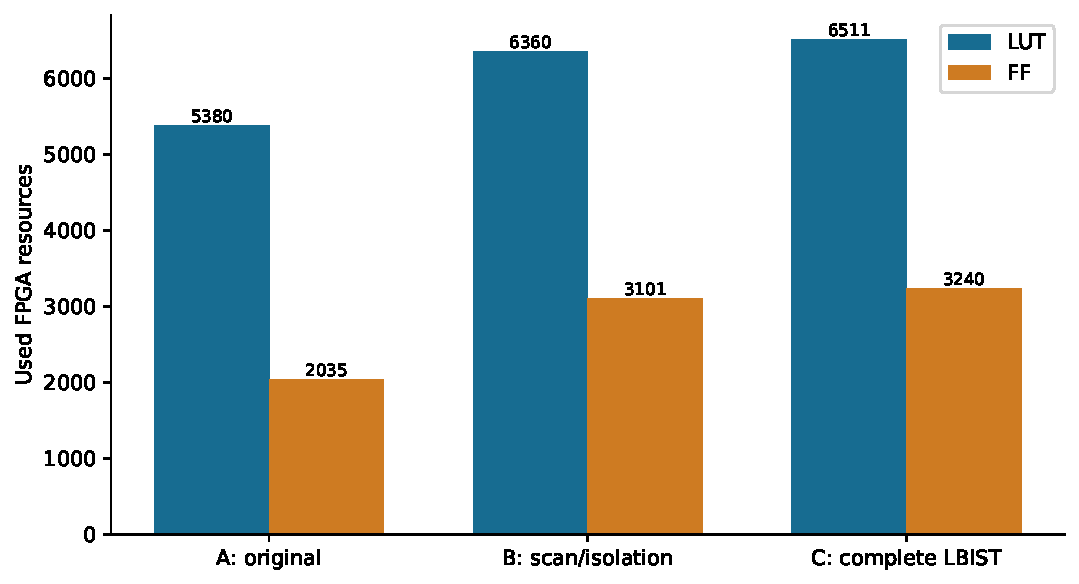
\includegraphics[width=\textwidth,height=.67\textheight,keepaspectratio]{FPGA_Analysis/figures/area_comparison.pdf}\caption{Area}\end{figure}


\begin{center}\resizebox{\textwidth}{!}{\begin{tabular}{llllll}\hline

\textbf{Comparison} & \textbf{LUT delta} & \textbf{LUT overhead (\%)} & \textbf{FF delta} & \textbf{FF overhead (\%)} & \textbf{Stage} \\\hline
Scan/isolation vs baseline & 980 & 18.2156 & 1066 & 52.3833 & Routed \\
Complete LBIST vs baseline & 1131 & 21.0223 & 1205 & 59.2138 & Routed \\
LBIST addition vs scan/isolation & 151 & 2.3742 & 139 & 4.4824 & Routed \\
\hline\end{tabular}}\end{center}


Overhead=(configuration-reference)/reference$\times$100, separately for LUT and FF. The B$\rightarrow$C row is incremental LBIST overhead; A$\rightarrow$B isolates scan/isolation overhead. Full resource counts include LUTRAM, carry, BRAM, DSP and clock primitives in \texttt{synthesis\_summary.csv}; LUT/FF utilization uses20,800/41,600 available. Primitive versus packed LUT counts can differ after physical optimization, so report\_utilization is the area-table authority. There is no single meaningful FPGA utilization percentage across unlike resources.



Baseline maps two RAMB18 primitives (one 36 Kb equivalent); B/C map no BRAM and use more FFs. Thus the large FF increase includes a storage-inference change in the existing isolation-helper implementation, not simply64 scan muxes. Wide observation ports are open and no debug bus is retained, but source coding/inference side effects are not eliminated by a memory refactor. These are the actual existing-implementation costs. They should not be interpreted as a technology-independent or memory-inference-neutral scan overhead.



\begin{center}\resizebox{\textwidth}{!}{\begin{tabular}{llllllll}\hline

\textbf{Configuration} & \textbf{Stage} & \textbf{WNS (ns)} & \textbf{TNS (ns)} & \textbf{WHS (ns)} & \textbf{Setup fails} & \textbf{Path (ns)} & \textbf{Closure} \\\hline
baseline & Routed & -77.054 & -5443.598 & -2.793 & 356 & 96.980 & FAIL \\
scan\_enabled & Routed & -77.212 & -7334.359 & -2.728 & 1157 & 97.136 & FAIL \\
full\_lbist & Routed & -76.315 & -7796.277 & -2.726 & 1278 & 96.283 & FAIL \\
\hline\end{tabular}}\end{center}


All reported50 MHz timing violations are retained. Successful synthesis, placement or routing does not imply timing closure. A maximum achievable frequency is not inferred from20 ns minusWNS because the worst path may cross phase-related clocks. No board operation or maximum frequency is established. Working RTL is preserved rather than altered to repair timing for this submission.



\subsection{Switching capture and estimated power}


The five LBIST approaches share \textbf{one implemented C netlist}. Each approach's exact production wrapper is simulated with its own real switching activity, fixed clock/pattern count/window and the same test environment. The router's unselected scheduling lanes use the same fixed production generics in every trace. A hierarchy-only SAIF mapping preserves all switching records and maps production instances to routed u\_system. MMCM/clock activity derives from timing constraints. RTL SAIF does not include routed glitches or establish gate-level timing behavior.



Actual C annotation is 1,963/14,106 design nets (13.9161\%) in each mode; Vivado reports Medium overall confidence. Remaining nets use propagation/default activity. Unknown-state warnings also occur on unused or uninitialized processor logic. The whole-C watt values below are therefore \textbf{assumption-dominated diagnostic estimates}, not a reliable whole-processor power-saving measurement. A and B have separate actual lwsw SAIF captures over 100--1670 ns; their partial mapping is 21.5681\% and 13.9894\%, respectively. Their dynamic estimates are 0.187 W and 0.163 W. Because storage inference and annotation differ, that difference is not evidence that adding scan lowers physical power. Vectorless initial reports remain separately labeled historical run artifacts.



\begin{center}\resizebox{\textwidth}{!}{\begin{tabular}{llllll}\hline

\textbf{Approach} & \textbf{WTM} & \textbf{Dynamic (W)} & \textbf{Shared LUT} & \textbf{Shared FF} & \textbf{WNS (ns)} \\\hline
Direct & 50.1154\% & 0.124 & 6511 & 3240 & -76.315 \\
Constant n=3 & 7.0665\% & 0.123 & 6511 & 3240 & -76.315 \\
Basic & 19.9764\% & 0.124 & 6511 & 3240 & -76.315 \\
Swap & 17.7531\% & 0.123 & 6511 & 3240 & -76.315 \\
Moving & 19.8701\% & 0.124 & 6511 & 3240 & -76.315 \\
\hline\end{tabular}}\end{center}


\begin{center}\resizebox{\textwidth}{!}{\begin{tabular}{llllllllll}\hline

\textbf{Approach} & \textbf{TotalW} & \textbf{StaticW} & \textbf{DynamicW} & \textbf{ClockW} & \textbf{LogicW} & \textbf{SignalsW} & \textbf{BRAMW} & \textbf{DSPW} & \textbf{MMCMW} \\\hline
Direct & 0.193 & 0.069 & 0.124 & 0.006 & 0.005 & 0.007 & 0.000 & 0.000 & 0.106 \\
Constant n=3 & 0.192 & 0.069 & 0.123 & 0.006 & 0.005 & 0.006 & 0.000 & 0.000 & 0.106 \\
Basic & 0.192 & 0.069 & 0.124 & 0.006 & 0.005 & 0.007 & 0.000 & 0.000 & 0.106 \\
Swap & 0.192 & 0.069 & 0.123 & 0.006 & 0.005 & 0.007 & 0.000 & 0.000 & 0.106 \\
Moving & 0.192 & 0.069 & 0.124 & 0.006 & 0.005 & 0.007 & 0.000 & 0.000 & 0.106 \\
\hline\end{tabular}}\end{center}


\begin{figure}[htbp]\centering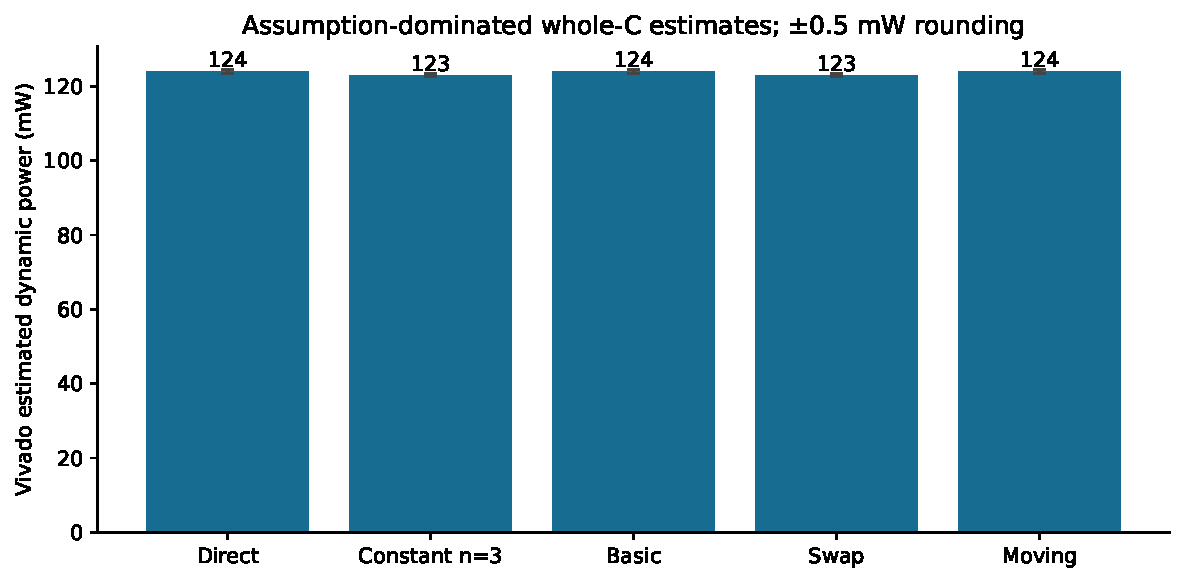
\includegraphics[width=\textwidth,height=.67\textheight,keepaspectratio]{FPGA_Analysis/figures/dynamic_power.pdf}\caption{Estimated dynamic power with rounding resolution}\end{figure}


\begin{figure}[htbp]\centering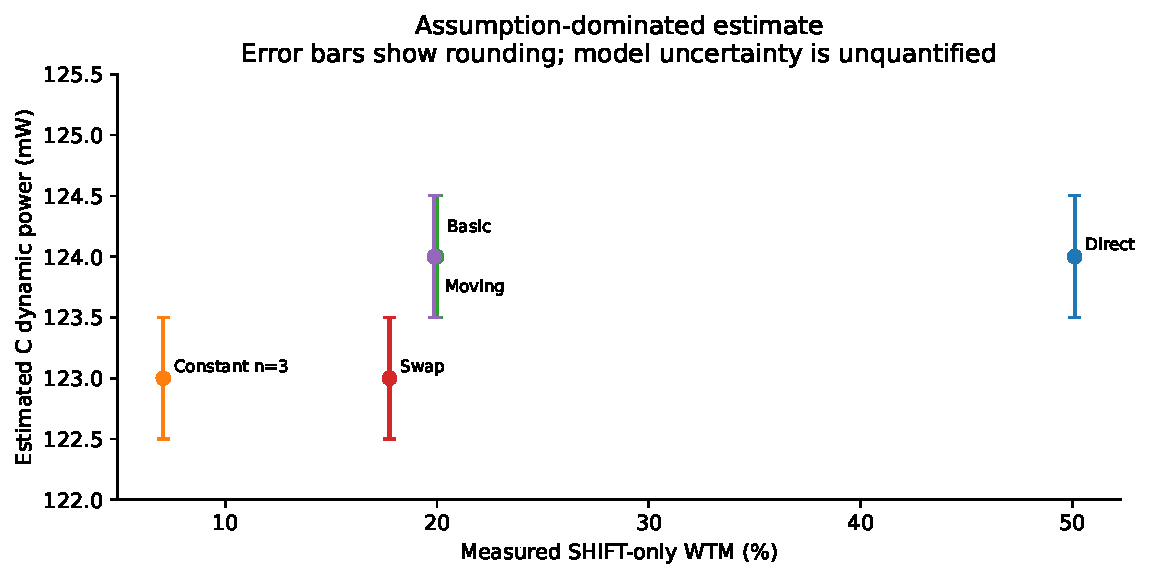
\includegraphics[width=\textwidth,height=.67\textheight,keepaspectratio]{FPGA_Analysis/figures/wtm_vs_power.pdf}\caption{WTM versus estimated power}\end{figure}


Error bars indicate only the 0.001 W report rounding ($\pm$0.0005 W), not model confidence bounds. Separate static/dynamic/total values are independently rounded and may not sum exactly. The common MMCM alone estimates 0.106 W, dwarfing the reported differences. No statistically or physically established power improvement is claimed from the 0.001 W mode differences.



As a limited fallback, the detailed reports retain the \textbf{same routed IF/RF hierarchy} across modes, including any synthesis-absorbed decode/comb logic. Direct reports0.002 W; other per-mode rows are not printed at the native report's hierarchy resolution and are explicitly marked unavailable. Router/controller/MISR source-tag counts and unmatched nets are retained separately; they are not extrapolated into missing watt values. Reliable finer subsystem power ranking and reliable whole-processor activity analysis remain unresolved limitations, rather than fabricated results. \texttt{power/subsystem\_comparison.csv} and \texttt{power/annotation\_by\_boundary.csv} preserve that boundary and availability.



WTM weights SHIFT transitions in 64 scanFFs. Vivado power includes clocks, processor logic, routing and other resources across SHIFT/CAPTURE/UNLOAD. WTM reduction therefore cannot be equated to total FPGA dynamic-power reduction. Power uses the selected part's default nominal supply assumptions and documented25$^\circ$C ambient/typical process settings when accepted by Vivado. It is an \textbf{estimated on-chip power study}, not physical board measurement. Timing failure at the requested frequency further limits interpreting these estimates as an operable hardware point. \texttt{FPGA\_Analysis/README.md} records exact mapping, confidence and run status.



All runs accept25$^\circ$C ambient and typical process. Native supplies include 1.0 V Vccint / Vccbram and 1.8 V Vccaux. Generic Vivado thermal defaults (medium board/heatsink, 250 LFM airflow) are consistent across runs and are not a calibrated Basys3 thermal model. External memory, package I/O and regulator/board losses are excluded. Initial reporting-call failures were repaired using saved checkpoints; all final seven SAIF power exports and five detailed exports completed. The C synthesis log's obsolete CONFIGURATION generic warning is retained: actual elaboration binds DESIGN\_CONFIG=2 and the post-route hierarchy check confirms the production router. The reproducible script uses the corrected generic name.



\subsection{Final timing-closure revision}


9.756097561 MHz is the highest tested common timing-clean OOC point. Board reference 100 MHz; M=8, common divider=82, VCO=800 MHz; period=102.5 ns. Related quarter-duty phases remain unchanged. A virtual CPU I/O reference corrects the old external launch-latency model. Actual failing input hold paths are repaired with checked physical identity LUT delays; original processor/LBIST RTL is unchanged. Automatic MMCM/device uncertainty is used, with no false paths added beyond asynchronous reset assertion.



\begin{center}\resizebox{\textwidth}{!}{\begin{tabular}{llllll}\hline

\textbf{Configuration} & \textbf{LUT} & \textbf{FF} & \textbf{Latches} & \textbf{BRAM36Equivalent} & \textbf{DSP} \\\hline
baseline & 5220 & 2008 & 0 & 1 & 7 \\
scan\_enabled & 6138 & 3084 & 0 & 0 & 7 \\
full\_lbist & 6243 & 3215 & 0 & 0 & 7 \\
\hline\end{tabular}}\end{center}


\begin{center}\resizebox{\textwidth}{!}{\begin{tabular}{lllllllll}\hline

\textbf{Configuration} & \textbf{FrequencyMHz} & \textbf{WNS} & \textbf{TNS} & \textbf{WHS} & \textbf{THS} & \textbf{SetupFails} & \textbf{HoldFails} & \textbf{TimingClean} \\\hline
baseline & 9.756098 & 0.154 & 0 & 0.069 & 0 & 0 & 0 & True \\
scan\_enabled & 9.756098 & 1.12 & 0 & 0.001 & 0 & 0 & 0 & True \\
full\_lbist & 9.756098 & 0.155 & 0 & 0.007 & 0 & 0 & 0 & True \\
\hline\end{tabular}}\end{center}


\begin{center}\resizebox{\textwidth}{!}{\begin{tabular}{lll}\hline

\textbf{Comparison} & \textbf{LUTPercent} & \textbf{FFPercent} \\\hline
Scan/isolation vs original & 17.5862 & 53.5857 \\
Full LBIST vs original & 19.5977 & 60.1096 \\
LBIST addition vs scan & 1.7107 & 4.2477 \\
\hline\end{tabular}}\end{center}


\begin{figure}[htbp]\centering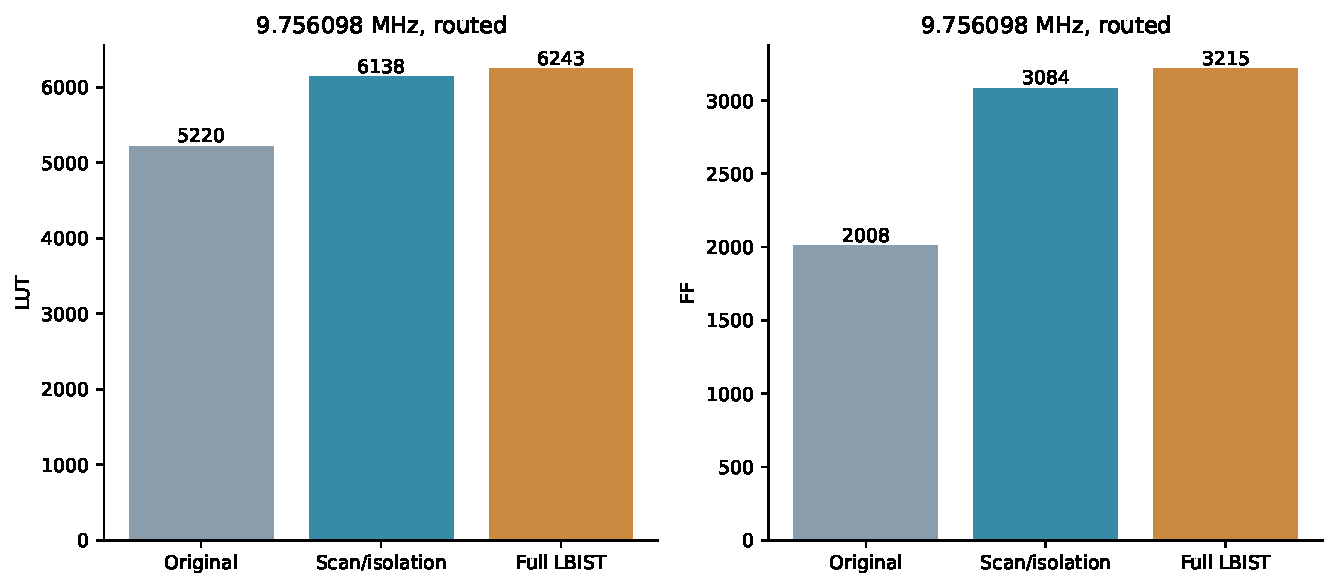
\includegraphics[width=\textwidth,height=.67\textheight,keepaspectratio]{FPGA_Analysis/Timing_Closure/figures/area_comparison.pdf}\caption{Updated area}\end{figure}


The initial large-divider 5/10 MHz attempts were rejected by real MMCM duty/phase limits, despite ideal clock reports. The corrected legal sweep, cross-phase results, all failed attempts and exact clock attributes are retained in the \href{FPGA_Analysis/Timing_Closure/README.md}{revision report}. No frequency is inferred from 1/(20 ns-WNS). This is the highest tested common OOC point when all three rows are timing-clean, not a global or board-qualified maximum. Vivado warns about unlocated OOC ports without HD.PARTPIN\_LOCS: external segments are not fully routed, and real external-interface timing is not established. The scan-enabled hold margin is only 0.001 ns. These results do not qualify a board implementation or supply additional timing margin.



Nine fresh simulations passed at this clock: real UNISIM phase/duty verification, original/scan lwsw with and without stalls, all five complete production streams and the original Basic fault 1. Independent checking confirms all 256 captures, each prefix signature and measured activity counts. Original 50 MHz fault-campaign data remains historical; no expanded fault universe or new whole-processor coverage claim is introduced. Payload time is 3.384960000 ms for 33,024 cycles. Updated execution times and activity windows are recorded separately.



\begin{center}\resizebox{\textwidth}{!}{\begin{tabular}{lllllll}\hline

\textbf{Approach} & \textbf{WTM} & \textbf{DynamicW} & \textbf{CommonLUT} & \textbf{CommonFF} & \textbf{AnnotationPercent} & \textbf{Confidence} \\\hline
Direct & 50.1154 & 0.099 & 6243 & 3215 & 13.4087 & Medium \\
Constant n=3 & 7.0665 & 0.099 & 6243 & 3215 & 13.4087 & Medium \\
Basic & 19.9764 & 0.099 & 6243 & 3215 & 13.4087 & Medium \\
Swap & 17.7531 & 0.099 & 6243 & 3215 & 13.4087 & Medium \\
Moving & 19.8701 & 0.099 & 6243 & 3215 & 13.4087 & Medium \\
\hline\end{tabular}}\end{center}


\begin{figure}[htbp]\centering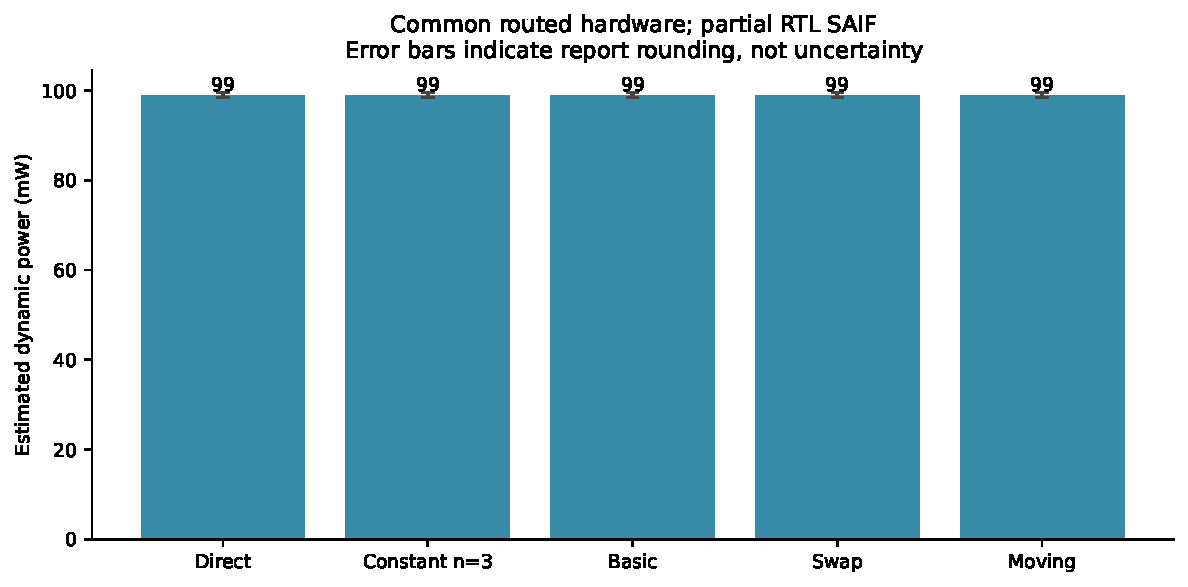
\includegraphics[width=\textwidth,height=.67\textheight,keepaspectratio]{FPGA_Analysis/Timing_Closure/figures/dynamic_power.pdf}\caption{Updated estimated power}\end{figure}


\begin{figure}[htbp]\centering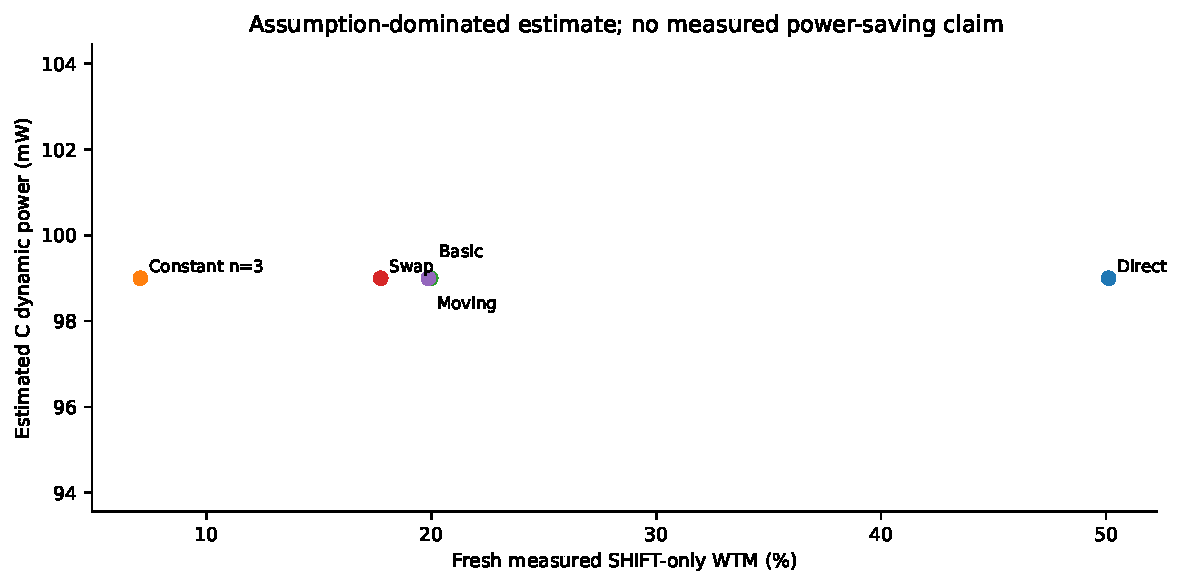
\includegraphics[width=\textwidth,height=.67\textheight,keepaspectratio]{FPGA_Analysis/Timing_Closure/figures/wtm_power.pdf}\caption{Fresh WTM versus estimated power}\end{figure}


Each power case uses fresh selected-clock activity on the same routed C netlist, not a 50 MHz SAIF reused with a new timing constraint. Partial matching and propagation/default assumptions remain visible; small 0.001 W report differences do not establish physical savings or a reliable ranking. Supply/ambient/process assumptions are consistent. All native utilization, timing, power, unmatched-net and register-Q annotation reports are available in Timing\_Closure. Clock-only source changes, physical repair cells, unsupported 5 MHz quarter-duty generation and OOC interface assumptions are fully documented there.





\section{Discussion and limitations}


The strongest result is reproducible control of scan switching with preserved capture ordering and safe completion handling on real cMIPS storage. The small fault universe saturates quickly and cannot distinguish coverage quality among the five approaches. It says little about random-pattern-resistant faults or broader datapath observability. The held instruction limits excitation, and only 64 of 720pipeline candidate bits are scanned. Other architectural state remains protected, not tested. A reset is required after destructive testing. Target quantization and finite sequence effects make measured WTM differ from theoretical targets. FPGA overhead depends on this virtual processor boundary and synthesis settings; the historical 50 MHz timing failure, current narrow OOC timing margins, external-interface assumptions and partial activity annotation must accompany the corresponding area/power figures. No 75\% whole-processor coverage, measured energy savings, silicon measurement, post-route functional equivalence or successful board deployment is claimed.



\section{Conclusion}


The final submission preserves the verified Phase6A LBIST architecture and consolidates native evidence, reproducible essential demonstrations and an explicit FPGA evaluation boundary. The primary256-pattern original16-fault comparison achieves12 detections per approach without observed final aliases, while measured scan WTM varies with filter/control choice. Safe MISR completion prevents aborted or incomplete streams from reporting MATCH. The available FPGA reports establish actual resource/timing/power estimates at their stated stages and limitations. Broader scan insertion, fault universes and physical measurement are deferred beyond this completed experimental scope.



\section{References}


1. T. Kato, S. Wang, Y. Sato, S. Kajihara and X. Wen, ``A Flexible Scan-in Power Control Method in Logic BIST and Its Evaluation with TEG Chips,'' IEEE Transactions on Emerging Topics in Computing,8(3),591--601,2020. \href{https://doi.org/10.1109/TETC.2017.2767070}{DOI10.1109/TETC.2017.2767070}; \href{https://kyutech.repo.nii.ac.jp/records/6935}{author repository record}. Paper results are distinct from this project's measurements.

2. R. A. Hexsel, cMIPS VHDL processor and documentation, supplied GPLv3 sources, \texttt{cMIPS/docs/cMIPS.pdf} and \texttt{cMIPS/vhdl/}.

3. Digilent, \href{https://digilent.com/reference/_media/basys3\%3A\%20basys3_rm.pdf}{Basys3 reference manual} and \href{https://github.com/Digilent/digilent-xdc/blob/master/Basys-3-Master.xdc}{official master XDC}. Used for target/100 MHz oscillator reference, not as an applied pinout in the virtual-I/O flow.

4. AMD Vivado2025.1.1 installed command help and native utilization/timing/power/switching reports under \texttt{FPGA\_Analysis/}; \texttt{device\_probe.log} records tool/part availability.

5. Repository experimental records, \texttt{Results/Phase1} (where present), \texttt{Results/Phase2}, \texttt{Results/Phase3}, \texttt{Results/Phase4}, \texttt{Results/Phase5A}, \texttt{Results/Phase5B}, \texttt{Results/Phase5 C}, \texttt{Results/Phase6A}, and final read-only audits. Earlier result directories remain authoritative historical evidence.



\section{Reproduction and evidence index}


See \href{README.md}{README}, \href{DEMO.md}{demo guide}, \href{final_verification_summary.md}{final verification summary}, \href{FPGA_Analysis/README.md}{FPGA study}, \href{final_experimental_comparison.csv}{primary comparison CSV}, and \href{source_manifest.csv}{source provenance}. Full per-fault tables are in \texttt{tables/}. Relevant actual waveform excerpts are \href{figures/scan_capture_unload.png}{capture/unload} and \href{figures/misr_abort.svg}{abort suppression}; the latter is copied unchanged from its VCD-verified historical figure. Native WDB/VCD/SAIF/checkpoints are local regenerable artifacts rather than required Git payloads.
\end{document}